\documentclass{beamer}

\usetheme{Madrid}      % 内置主题(推荐新手使用)
\useoutertheme{miniframes} % 外层主题:横向小方块目录条
% \usetheme{Frankfurt}
% \usepackage[x11names]{xcolor}  % 加载扩展色库
% \usecolortheme[named=OliveDrab3]{structure}  % 柔和绿色

\title{Wavelet Transform for Image Processing}
\author{
\texorpdfstring{
Zhang Jinrui\thanks{alternative email:zhangjr1022@mails.jlu.edu.cn}
\\
He Jiashun
\\
Meng Jingyuan
\\
Jiang Zishen
\\
Mo Zian
}
{
Zhang Jinrui\thanks{alternative email:zhangjr1022@mails.jlu.edu.cn}
,
He Jiashun
,
Meng Jingyuan
,
Jiang Zishen
,
Mo Zian
}
}
\date{\today}

\begin{document}

\frame{\titlepage}  % 首页封面

\section{Pre-Processing}
\begin{frame}
    \frametitle{Pre}

    To transform a image into \(2^N \times 2^N\)

    sadfsa
    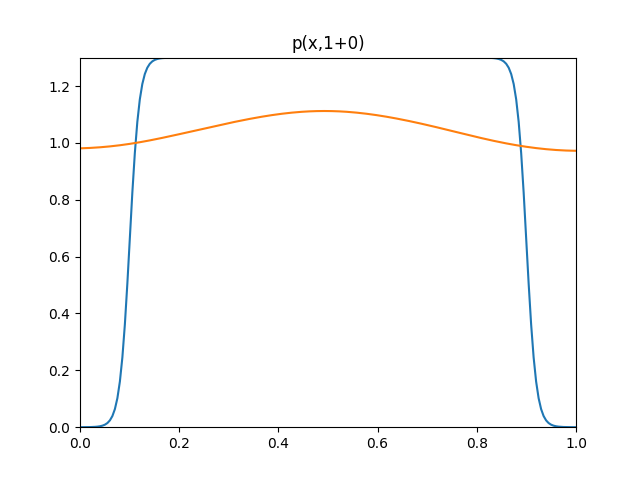
\includegraphics[width=0.5\textwidth]{fig/p(x,1+0).png}
    \pause

    sdfas
    \[
        E = mc^2
    \]
\end{frame}

\begin{frame}
    \frametitle{sadf}
    \begin{itemize}[<+->]
        \item sadf
        \item sadf
        \item sdgas
    \end{itemize}
\end{frame}

\begin{frame}
    \frametitle{Basic Idea}
    Vector decomposition.
\end{frame}

\section{Haar Compression}
\begin{frame}
    \frametitle{Standard Haar Decomposition}
    \begin{itemize}
        \item sdlfkj
        \item sDF
        \item sdf
    \end{itemize}
\end{frame}
\begin{frame}
    \frametitle{sfdfg}
    \begin{itemize}
        \item sdlfkj
        \item sDF
        \item sdf
    \end{itemize}
\end{frame}
\begin{frame}
    \frametitle{sadsgkjh}
    \begin{itemize}
        \item sdlfkj
        \item sDF
        \item sdf
    \end{itemize}
\end{frame}
\begin{frame}
    \frametitle{sdf}
    \begin{itemize}
        \item sdlfkj
        \item sDF
        \item sdf
    \end{itemize}
\end{frame}

\section{Haar Compression Augmented}
\begin{frame}
    \frametitle{second title}
    \begin{itemize}
        \item sdlfkj
        \item sDF
        \item sdf
    \end{itemize}
\end{frame}
\begin{frame}
    \frametitle{sfdfg}
    \begin{itemize}
        \item sdlfkj
        \item sDF
        \item sdf
    \end{itemize}
\end{frame}

\section{Zishen Jiang}
\begin{frame}
    \frametitle{sadsgkjh}
    \begin{itemize}
        \item sdlfkj
        \item sDF
        \item sdf
    \end{itemize}
\end{frame}

\section{Energy Analysis}
\begin{frame}
    \frametitle{sdf}
    \begin{itemize}
        \item sdlfkj
        \item sDF
        \item sdf
    \end{itemize}
\end{frame}

\end{document}
